\section{ACTIVIDAD PRÁCTICA SOBRE SCR} 
\subsection{Condición de disparo $I_G$ y corriente de mantenimiento $I_H$}
\sangria{} El objetivo de esta actividad es determinar la polarización y le funcionamiento del SCR, tanto en una etapa de simulación como en la correspondiente implementación.\\
\midTitle{teal}{Circuito para polarización}{}
\begin{center}\begin{tikzpicture}
	% Paths, nodes and wires:
	\draw (1.25, 7.75) to[american voltage source, l={$20V$}] (1.25, 5);
	\draw (3.58, 8.349) to[american resistor, l={$R_1 = 3,3k\Omega$}] (3.58, 6.349);
	\draw (3.58, 4.099) to[variable american resistor, l={$\text{POT  } 5k\Omega$}] (3.58, 6.349);
	\draw (1.25, 5) -- (1.25, 2.75) -- (4, 2.75) -- (4.25, 2.75);
	\node[ground] at (1.25, 2.75){};
	\draw (4, 5) to[american resistor, l={$R_3 = 4,7 k\Omega$}] (6.5, 5);
	\draw (6.75, 4.5) to[voltmeter, l={$V_G$}] (6.75, 2.75);
	\draw (4.25, 2.75) -- (8.5, 2.75);
	\draw (6.75, 5) to[ammeter, l={$I_G$}] (9.75, 5);
	\draw (9.719, 5) to[cute closing switch] (11.969, 5);
	\draw (12.77, 7.2) to[stroke thyristor, mirror] (12.77, 4.2);
	\draw (12.77, 7.2) to[american resistor, l={$R_4 = 4,7k\Omega$}] (12.77, 9.45);
	\draw (14.5, 7) to[voltmeter, l={$V_{AK}$}] (14.5, 4);
	\draw (12.77, 4.2) to[ammeter, l={$I_{AK}$}] (12.75, 2.75);
	\draw (8.5, 2.75) -- (14.25, 2.75);
	\draw (17.25, 6.75) to[american voltage source, l={$V_{cc}$}] (17.25, 4);
	\draw (3.58, 3.099) |- (3.5, 2.75);
	\draw (3.58, 8.349) -| (1.25, 7.75);
	\draw (3.58, 4.099) -- (3.58, 3.099);
	\draw (6.5, 5) -- (6.75, 5);
	\draw (6.75, 5) -| (6.75, 4.5);
	\draw (11.969, 5) -- (12, 5);
	\draw (16, 8.25) to[voltmeter, l={$V_{cc}$}] (16, 5.25);
	\draw (14.25, 2.75) -| (14.5, 4);
	\draw (12.77, 7.2) -| (14.5, 7);
	\draw (12.75, 9.5) -| (16, 8.25);
	\draw (17.25, 6.75) |- (16, 9.5);
	\draw (16, 5.25) |- (14.5, 2.75);
	\draw (17.25, 4) |- (16, 2.75);
\end{tikzpicture}\end{center}
\subsubsection{Actividad de laboratorio}
\midTitle{red}{Armado de circuito}{}
\begin{center}
    \tikzset{
          hole/.style = {fill = #1, circle, minimum width = 1mm, inner sep = 0mm},
          wire/.style = {draw = #1, line width = 0.2mm},
          label/.style = {rotate = 0, black!50!white, font=\sffamily, anchor = center}
        }
        \begin{tikzpicture}[x=2mm,y=2mm]
          \draw[fill=black!05!white] (-32,-4) rectangle (1,16);
 
          \foreach \yi in {1,...,30}{
            \node[hole=red]  at (-\yi,-3){};
            \node[hole=blue] at (-\yi,-2){};
            \node[hole=red]  at (-\yi,14){};
            \node[hole=blue] at (-\yi,15){};
            \foreach \xs in {0,6}{
                \foreach \xi in {1,2,3,4,5}{
                    \node[hole=black] at (-\yi,\xi+\xs){};
                }
            }
        }
        \foreach \m/\xi in {A/1,B/2,C/3,D/4,E/5,F/7,G/8,H/9,I/10,J/11}{
            \node[label=0] at (0,\xi) {\tiny\m};
            \node[label=0] at (-31,\xi) {\tiny\m};
        }
        \foreach \n/\yi in {1,5,10,15,20,25,30}{
            \node[label=0] at (-\yi,-1) {\tiny\n};
            \node[label=0] at (-\yi,13) {\tiny\n};
        }
        \filldraw[line width=1.5pt, fill=orange!25] (-40, 20) circle (0.60cm);
        \draw[line width=1.5pt, blue!90] (-40, 23) -- (-40, 25) -- (-30, 25) -- (-30, 15);
        \draw[line width=1.5pt, red!90] (-40, 17) -- (-40, 14) -- (-30, 14);
        \node at (-40, 18) {\large\textbf{+}};
        \node at (-40, 22) {\large\textbf{-}};
        \node at (-34, 20) {\Large\textbf{$20V$}};
        \filldraw[line width=0.5pt, fill=brown!60] (-28.5, 11) rectangle (-27.5, 13.25);
        \filldraw[line width=0.25pt, draw=black, fill=orange!80] (-28.5, 11.25) rectangle (-27.5, 11.5);
        \filldraw[line width=0.25pt, draw=black, fill=red!80] (-28.5, 11.75) rectangle (-27.5, 12);
        \filldraw[line width=0.25pt, draw=black, fill=red!80] (-28.5, 12.25) rectangle (-27.5, 12.5);
        \filldraw[line width=0.25pt, draw=black, fill=gold!80] (-28.5, 12.75) rectangle (-27.5, 13);
        \draw[line width=1pt, draw=black!60] (-28, 13.25) -- (-28, 14);
        \draw[line width=1pt, draw=black!60] (-28, 11) -- (-28, 10);
        \filldraw[line width=0.5pt, draw=black, fill=brown!60, rounded corners=3pt] (-29, 9.5) rectangle (-23, 7);
        \filldraw[line width=0.5pt, draw=black, fill=brown!70] (-29, 7.35) rectangle (-23, 6.5);
        \draw[line width=1pt, draw=blue!90] (-24, 11) -- (-24, 15);
        \filldraw[line width=0.5pt, draw=black, fill=gray!90] (-28, 6.5) rectangle (-24, 6);
        \filldraw[line width=0.5pt, draw=black, fill=gray!70] (-26.5, 6) rectangle (-25.5, 3.5);
        \draw[line width=1.25pt, draw=black!70] (-26, 6) -- (-26, 3.5);
       

       \draw[line width=1pt, draw=black!60] (-26, 10) -- (-23, 10);
       \filldraw[line width=0.5pt, draw=black, fill=brown!60] (-23, 10.5) rectangle (-20.75, 9.5);
       \filldraw[line width=0.25pt, draw=black, fill=yellow] (-22.75, 10.5) rectangle (-22.5, 9.5);
       \filldraw[line width=0.25pt, draw=black, fill=violet] (-22.25, 10.5) rectangle (-22, 9.5);
       \filldraw[line width=0.25pt, draw=black, fill=red] (-21.75, 10.5) rectangle (-21.5, 9.5);
       \filldraw[line width=0.25pt, draw=black, fill=gold] (-21.25, 10.5) rectangle (-21, 9.5);
    \draw[line width=1pt, draw=black!60] (-20.75, 10) -- (-20, 10);
    \filldraw[line width=0.5pt, draw=black, fill=black!80] (-17.5, 8) rectangle (-14.5, 9.25);
    \filldraw[line width=0.5, draw=black, fill=gray!70] (-17.5, 8) rectangle (-14.5, 7.5);
    \draw[line width=1pt, draw=red] (-17, 7) -- (-20, 7);
    \draw[line width=1pt, draw=blue!90] (-15, 11) -- (-15, 15);
    \draw[line width=1pt, draw=black!60] (-16, 10) -- (-14, 10);
       \filldraw[line width=0.5pt, draw=black, fill=brown!60] (-14, 10.5) rectangle (-11.75, 9.5);
       \filldraw[line width=0.25pt, draw=black, fill=yellow] (-13.75, 10.5) rectangle (-13.5, 9.5);
       \filldraw[line width=0.25pt, draw=black, fill=violet] (-13.25, 10.5) rectangle (-13, 9.5);
       \filldraw[line width=0.25pt, draw=black, fill=red] (-12.75, 10.5) rectangle (-12.5, 9.5);
       \filldraw[line width=0.25pt, draw=black, fill=gold] (-12.25, 10.5) rectangle (-12, 9.5);
       \draw[line width=1pt, draw=black!60] (-11.75, 10) -- (-10, 10);
       \draw[line width=1.5pt, draw=red] (-10, 11) -- (-10, 18) -- (5, 18);
       \draw[line width=1.5pt, draw=blue] (7, 18) -- (12, 18) -- (12, 13) -- (0, 13) -- (0, 15) -- (-1, 15);
        \filldraw[line width=1.5pt, fill=orange!25] (5, 18) circle (0.60cm);
        \node at (3, 18) {\large\textbf{+}};
        \node[rotate=90] at (7, 18) {\large\textbf{-}};
        \node at (4.75, 23) {\Large\textbf{$V_{CC}$}}; 
\end{tikzpicture}
\end{center}
\imagen[Fotografía del circuito]{10cm}{./imagenes/actividadSCR/protoboardCircuito.jpg}
\imagen[Pines del SCR BT151]{8cm}{./imagenes/pinesBT151.png}


\midTitle{red}{Flujo de trabajo}{}
\usetikzlibrary{shapes.geometric, arrows.meta, positioning}

\tikzstyle{block} = [rectangle, rounded corners, align=center,minimum width=1cm, minimum height=1cm,
text centered, draw=black, fill=gray!10]
\tikzstyle{arrow} = [thick, -{Stealth[length=3mm]}]

\begin{center}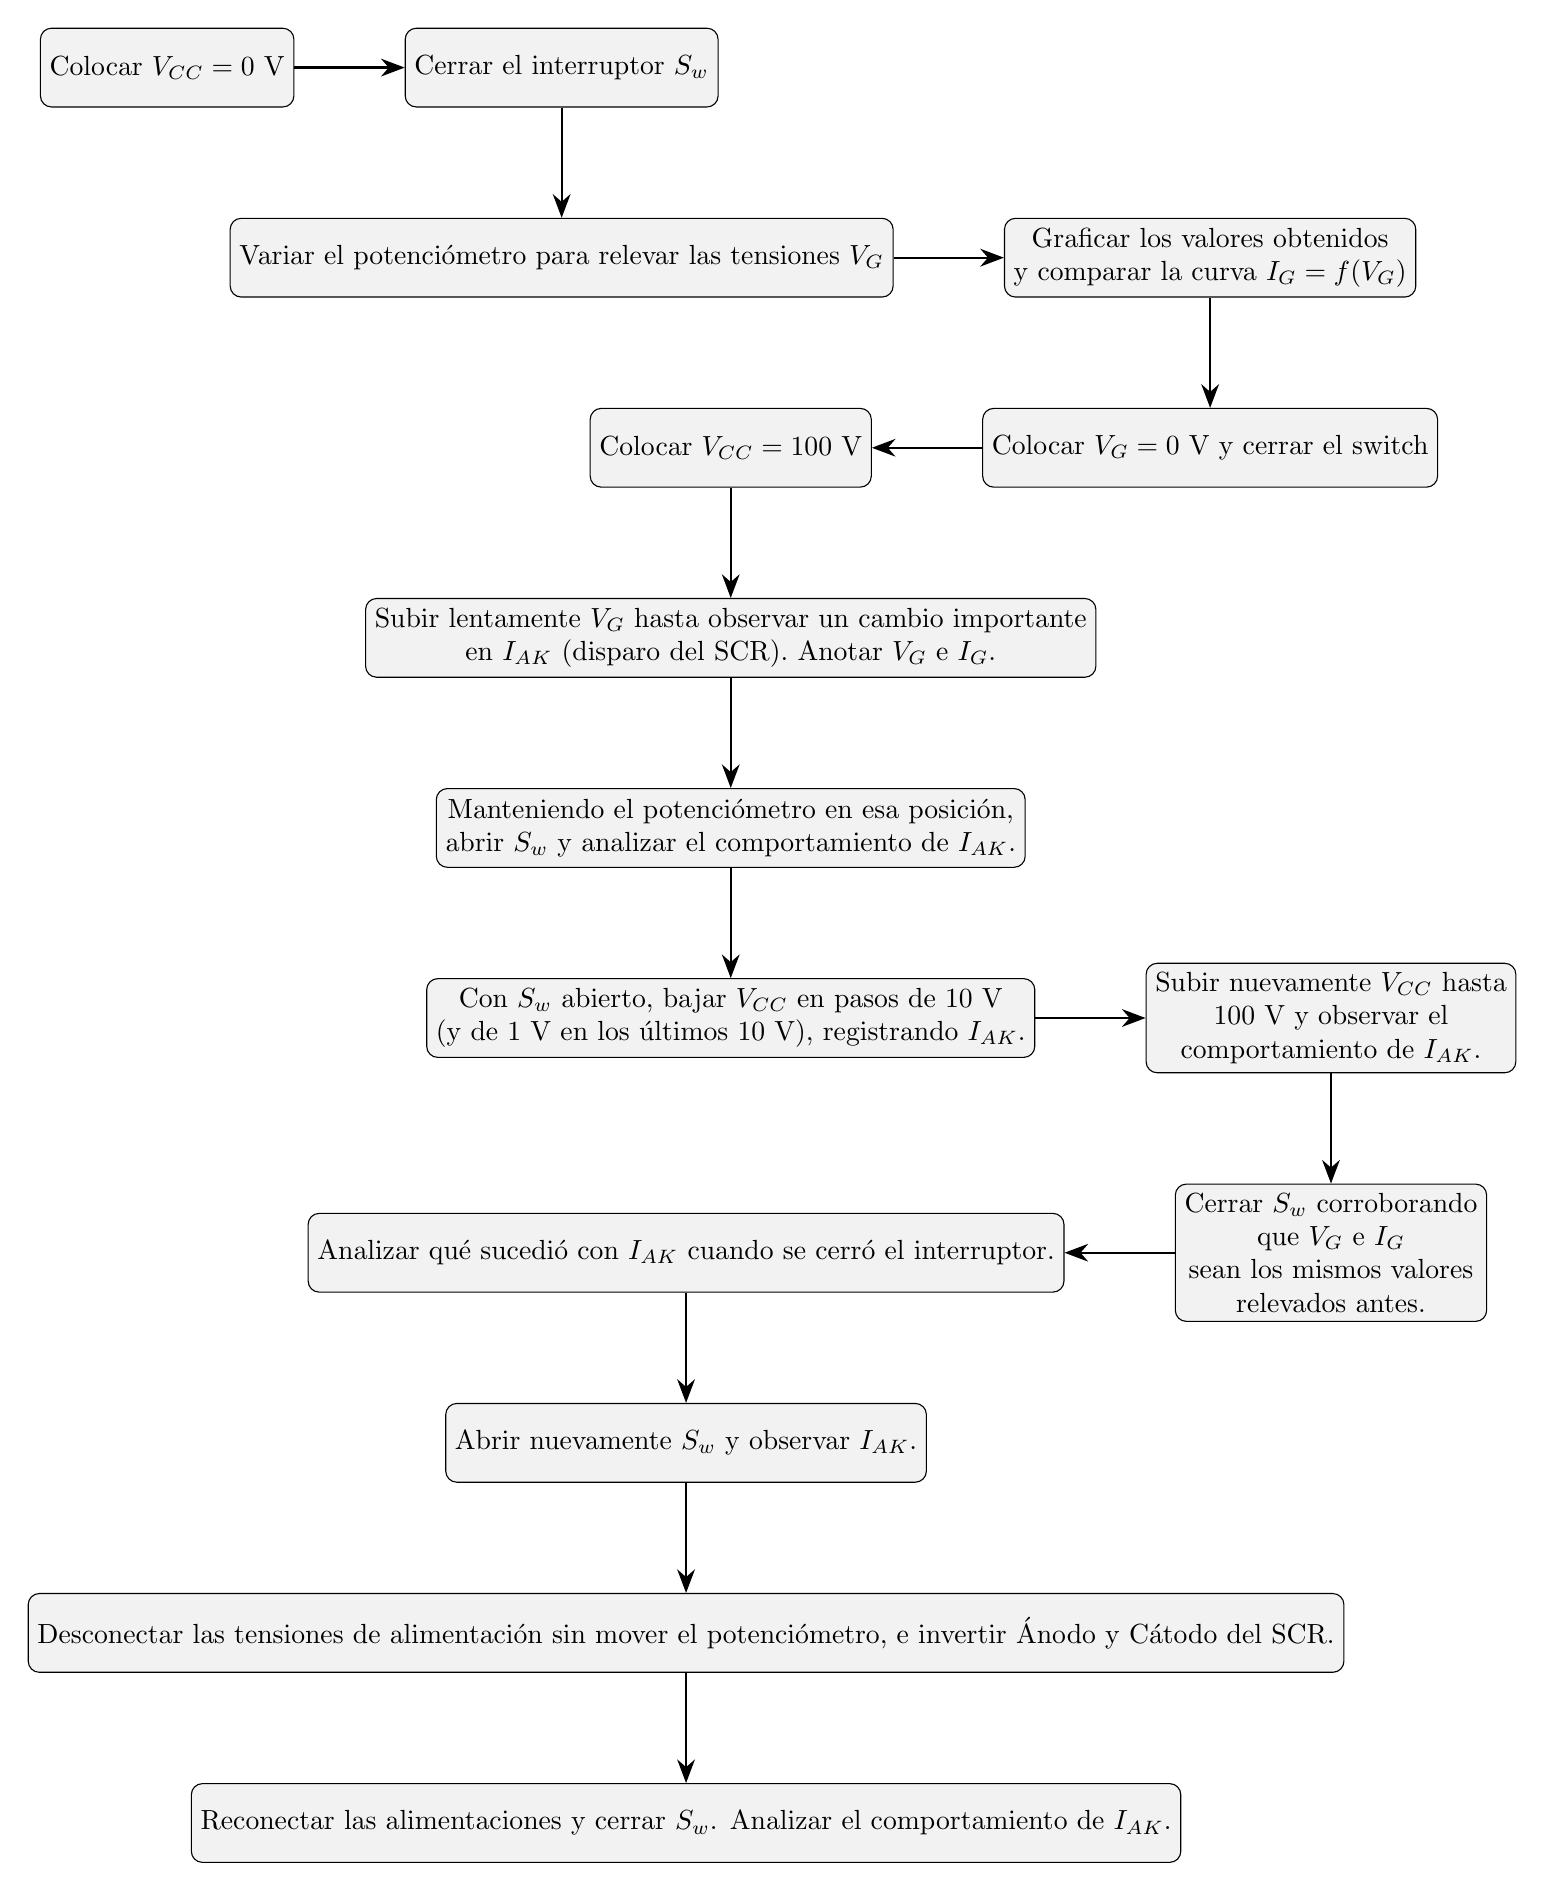
\begin{tikzpicture}[node distance=1.4cm]

\node (2) [block] {Colocar $V_{CC}=0$ V};
\node (3) [block, right=of 2] {Cerrar el interruptor $S_w$};
\node (4) [block, below=of 3] {Variar el potenciómetro para relevar las tensiones $V_G$};
\node (5) [block, right=of 4] {Graficar los valores obtenidos \\y comparar la curva $I_G = f(V_G)$};
\node (6) [block, below=of 5] {Colocar $V_G = 0$ V y cerrar el switch};
\node (7) [block, left=of 6] {Colocar $V_{CC} = 100$ V};
\node (8) [block, below=of 7] {Subir lentamente $V_G$ hasta observar un cambio importante\\ en $I_{AK}$ (disparo del SCR). Anotar $V_G$ e $I_G$.};
\node (9) [block, below=of 8] {Manteniendo el potenciómetro en esa posición, \\abrir $S_w$ y analizar el comportamiento de $I_{AK}$.};
\node (10) [block, below=of 9] {Con $S_w$ abierto, bajar $V_{CC}$ en pasos de 10 V \\(y de 1 V en los últimos 10 V), registrando $I_{AK}$.};
\node (11) [block, right=of 10] {Subir nuevamente $V_{CC}$ hasta \\ 100 V y observar el \\comportamiento de $I_{AK}$.};
\node (12) [block, below=of 11] {Cerrar $S_w$ corroborando \\que $V_G$ e $I_G$ \\sean los mismos valores\\ relevados antes.};
\node (13) [block, left=of 12] {Analizar qué sucedió con $I_{AK}$ cuando se cerró el interruptor.};
\node (14) [block, below=of 13] {Abrir nuevamente $S_w$ y observar $I_{AK}$.};
\node (15) [block, below=of 14] {Desconectar las tensiones de alimentación sin mover el potenciómetro, e invertir Ánodo y Cátodo del SCR.};
\node (16) [block, below=of 15] {Reconectar las alimentaciones y cerrar $S_w$. Analizar el comportamiento de $I_{AK}$.};

\foreach \i [evaluate=\i as \j using int(\i+1)] in {2,...,15}
    \draw [arrow] (\i) -- (\j);

\end{tikzpicture}
\end{center}

\midTitle{blue}{Preguntas}{}
\begin{itemize}[nosep]
    \item \textbf{Analizar y mencionar la alternativa que se presentó para disparar un SCR ¿Cómo la puede explicar? Existe otra manera de disparar el SCR sin corriente en la compuerta ¿Cual es ese método?}
\end{itemize}
\sangria{} El método de disparo que se usó al principio fue hacer variar la corriente $I_G$ para que el SCR se ''encienda'', usando como variador el potenciometro (menos resistencia $\rightarrow$ más corriente en $Gate$).
\imagen[Curvas IG-VG teoría]{15cm}{./imagenes/actividadSCR/curvasDelSCRGuanuco.png}
\sangria{} Con una $V_G$ constante, haciendo variar el potenciometro, se modifica el valor de la corriente en $Gate$ por lo que el SCR se activa según la gráfica $a)$. Esto se puede comprobar midiendo $I_{AK}$, que pasa de unos $\mu A$ y bruscamente unos $mA$. \\
\sangria{} Con el potenciometro fijo, se puede activar el SCR subiendo la tensión de $Gate$, tal como expone el gráfico $b)$. Es decir, se puede tener un valor fijo del potenciometro y con variar la tención se logra alcanzar el valor de $V_{BR}$ donde el tiristor pasa de polarización bloqueo en directa, a polarización conduccion en directa.
\begin{itemize}
\item \textbf{Analizar y sacar conclusiones de las conexiones y mediciones realizadas}
\end{itemize}
\sangria{} Viendo las gráficas, podemos concluir que más allá de un arreglo de tensiones y/o corrientes, activar el SCR significa que debemos inyectar una potencia tal en el $Gate$ para que esto suceda. Dicho valor es un punto en la pendiente.

% No conclusion?

% ###########################################################################################################################
% ###########################################################################################################################
% ##########################################+###########################################++++++###############################
% ####################################+++#++###########################################++++++++##############################
% ###################################+++++++++++++###+++++##########################++++++++++++#############################
% ###################################++++++++++++++++++++++++++++######+#############++++++++++++############################
% ###################################++++++++++++++++++++++++++++++++++++#++#########++++++++++++############################
% ##################################++++++++++++++++++++++++++++++++++++++++++##+++++++++++++++++############################
% ##################################+++++++++++++++++++++++++++++++++++++++++++++++++++++++++++++############################
% ##################################+++++++++++++++++++++++++++++++++++++++++++++++++++++++++++++############################
% #################################+++++++++++++++++++++++++++++++++++++++++++++++++++++++++++++#############################
% #################################+++++++++++++++++++++++++++++++++++++++++++++++++++++++++++++#############################
% ################################+++++++++++++++++++++++++++++++++++++++++++++++++++++++++++++##############################
% ################################++++++++++####+++++++++++++++++++++++++++++++++++++++++++++++##############################
% ################################++++##########+++#++++++++++++++++++++++++++++++++++++++++++###############################
% #############################################++++###+++++++++++++++++++++++++++++++++++++++################################
% ###########################################++++++++#####++++++++++++++++++++++++++++++++++#################################
% #####################################++++++++++++++++#################+++++++++++++++++++##################################
% ####################################+++++++++++++++++++#################++++++++++++++++###################################
% #####################################++++++++++++++++++++++##############+++++++++++++#####################################
% #######################################+++#####++++++++++++++++++#########+++++++++++######################################
% #################################################++#+++#######++++++######++++++++#########################################
% #########################################+++#####++###############+++++###++++++###########################################
% #########################################-++###+#++#################++++##++++++#+++#######################################
% #########################################++######++######+++#############+++++#############################################
% ##########################################++#####++#####+++##############++++##+###########################################
% #######################################++#######+++#####+++#######+##++++++################################################
% #######################################++++##+++++######+++######++#+++++++#+##############################################
% ########################################+++++++++#########++#######++++++++################################################
% ########################################++++++++##################+++++++##################################################
% ########################################+#++++++####++#########+++++++++###################################################
% #########################################++++++++++++##++++++++++++++++####################################################
% ########################################+++++++++++++++++########+++++###+#########+#######################################
% #######################################++++++++++++++++##########++++#++###########+#######################################
% #######################################++++++++++++++++########++++++######################################################
% ######################################++++++++-+++++++########++++++#######################################################
% ####################################++++++++-++++++++########++++++########################################################
% #####################################+++++++++++++++++++####++++++#########################################################
% ######################################+++++++++++++++++++###+++++##########################################################
% #########################################+#####+++++++++++#+++++###########################################################
% #########################################+######++++++#+++#++++############################################################
% #########################################+#########+++++#+#+++#############################################################
% ###########################################################################################################################
% ###########################################################################################################################

\begin{center}
\begin{tabular}{|c|c|c|}
\hline
\rowcolor[HTML]{FFFFC7} 
$V_{CC}$ {[}V{]} & $V_{AK}$ {[}V{]} & $I_{AK}$ {[}A{]} \\ \hline
100              & 730m             & 21,1m            \\
90               & 729m             & 18,7m            \\
80               & 726m             & 16,6m            \\
70               & 724m             & 14,5m            \\
60               & 721m             & 12,4m            \\
50               & 721m             & 10,3m            \\
40               & 728m             & 8,2m             \\
35               & 742m             & 7,2m             \\
30               & 805m             & 6m               \\
28.4             & 28.4             & 0                \\ \hline
\end{tabular}
\end{center}

\begin{center}
\begin{tabular}{c|cccccccccc}
\hline
\rowcolor[HTML]{FFFFC7} 
\cellcolor[HTML]{FFCE93}$V_G$ {[}V{]} & 0.2      & 0.3      & 0.4       & 0.5       & 0.6    & 0.7    & 0.8    & 0.9 & 1 & 1.1 \\ \hline
\cellcolor[HTML]{FFCE93}$I_G$ {[}A{]} & $634\mu$ & $936\mu$ & $1266\mu$ & $1588\mu$ & $233m$ & $281m$ & $313m$ & -   & - & -   \\ \hline
\end{tabular}
\end{center}
\imagen[Curva $I_G = f(V_G)$]{10cm}{./imagenes/actividadSCR/curvasDelSCRNosotros.png}

\subsubsection{Actividad de simulación}
\midTitle{teal}{Circuito para la simulación}{}
\begin{center}
\begin{tikzpicture}
	% Paths, nodes and wires:
	\draw (4.25, 5.5) to[american voltage source, l={$V_1$}] (4.25, 4);
	\draw (5, 5.5) to[american resistor, l={$R_2 = 4,7k\Omega$}] (7.5, 5.5);
	\draw (8.27, 7.325) to[empty thyristor, mirror] (8.27, 5.075);
	\draw (8.27, 7.325) to[american resistor, l={$R_1 = 4,7k\Omega$}] (8.25, 9.25);
	\draw (10.25, 5.5) to[american voltage source, l={$V_2$}] (10.25, 4);
	\node[ground] at (4.25, 4){};
	\node[ground] at (8.25, 4){};
	\node[ground] at (10.25, 4){};
	\draw (8.25, 4) -| (8.27, 5.075);
	\draw (4.25, 5.5) -- (5, 5.5);
	\draw (10.25, 5.5) |- (8.25, 9.25);
\end{tikzpicture}\end{center}

\midTitle{red}{Flujo de trabajo}{}

{

\tikzstyle{block} = [rectangle, rounded corners,
                     draw=black, fill=gray!10,
                     text width=8cm, minimum height=1cm,
                     align=center, font=\small]

\tikzstyle{arrow} = [thick, -{Latex[length=3mm,width=2mm]}]
\begin{center}
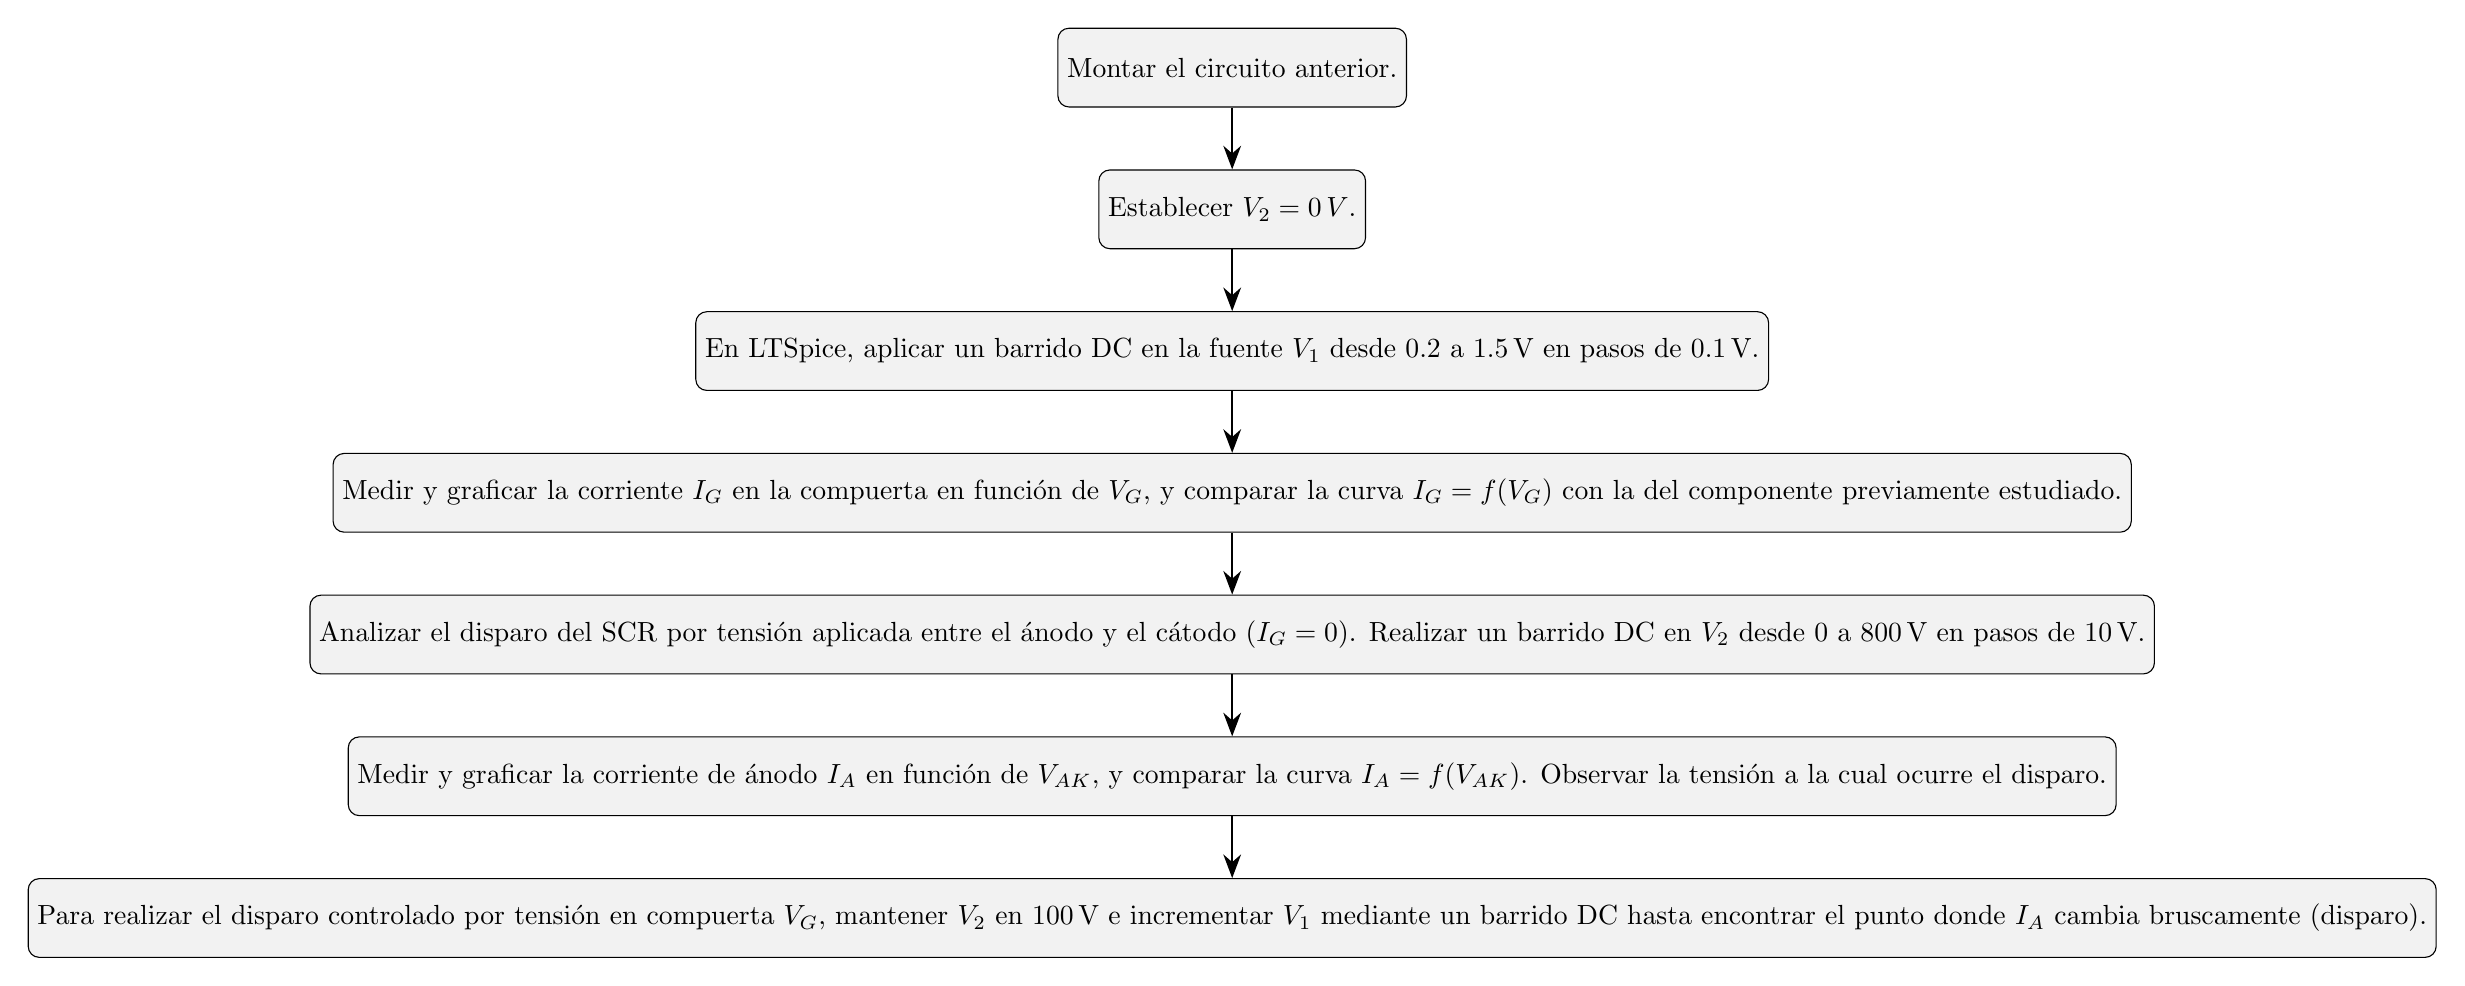
\begin{tikzpicture}[node distance=1.8cm]

\node[block] (a) {Montar el circuito anterior.};
\node[block, below of=a] (b) {Establecer $V_2 = 0\,\text{V}$.};
\node[block, below of=b] (c) {En LTSpice, aplicar un barrido DC en la fuente $V_1$ desde $0.2$ a $1.5$\,V en pasos de $0.1$\,V.};
\node[block, below of=c] (d) {Medir y graficar la corriente $I_G$ en la compuerta en función de $V_G$, y comparar la curva $I_G = f(V_G)$ con la del componente previamente estudiado.};
\node[block, below of=d] (e) {Analizar el disparo del SCR por tensión aplicada entre el ánodo y el cátodo ($I_G = 0$). Realizar un barrido DC en $V_2$ desde $0$ a $800$\,V en pasos de $10$\,V.};
\node[block, below of=e] (f) {Medir y graficar la corriente de ánodo $I_A$ en función de $V_{AK}$, y comparar la curva $I_A = f(V_{AK})$. Observar la tensión a la cual ocurre el disparo.};
\node[block, below of=f] (g) {Para realizar el disparo controlado por tensión en compuerta $V_G$, mantener $V_2$ en $100$\,V e incrementar $V_1$ mediante un barrido DC hasta encontrar el punto donde $I_A$ cambia bruscamente (disparo).};

\draw[arrow] (a) -- (b);
\draw[arrow] (b) -- (c);
\draw[arrow] (c) -- (d);
\draw[arrow] (d) -- (e);
\draw[arrow] (e) -- (f);
\draw[arrow] (f) -- (g);
\end{tikzpicture} 

\end{center}}
\imagen[Curva $I_G = f(V_G)$ LtSpice]{10cm}{./imagenes/actividadSCR/curvasIgFuncionVgSimulacion.png}
\imagen[Curva $I_A = f(V_{AK})$ LtSpice]{16cm}{./imagenes/actividadSCR/I_A-en-funcion-V_AK.png}
\subsection{Obtención de curvas característica del SCR}
\sangria{} El objetivo de esta actividad es lograr un relevamiento de los puntos de trabajo para graficar las curvas características.

\midTitle{teal}{Circuito para curvas características}{}
\begin{center}\begin{tikzpicture}
	% Paths, nodes and wires:
	\draw (1.25, 7.75) to[american voltage source, l={$20V$}] (1.25, 5);
	\draw (3.58, 8.349) to[american resistor, l={$R_1 = 3,3k\Omega$}] (3.58, 6.349);
	\draw (3.58, 4.099) to[variable american resistor, l={$\text{POT  } 5k\Omega$}] (3.58, 6.349);
	\draw (1.25, 5) -- (1.25, 2.75) -- (4, 2.75) -- (4.25, 2.75);
	\node[ground] at (1.25, 2.75){};
	\draw (4, 5) to[american resistor, l={$R_3 = 4,7 k\Omega$}] (6.5, 5);
	\draw (6.75, 4.5) to[voltmeter, l={$V_G$}] (6.75, 2.75);
	\draw (4.25, 2.75) -- (8.5, 2.75);
	\draw (6.75, 5) to[ammeter, l={$I_G$}] (9.75, 5);
	\draw (12.77, 7.2) to[stroke thyristor, mirror] (12.77, 4.2);
	\draw (12.77, 7.2) to[american resistor, l={$R_4 = 4,7k\Omega$}] (12.77, 9.45);
	\draw (14.5, 7) to[voltmeter, l={$V_{AK}$}] (14.5, 4);
	\draw (12.77, 4.2) to[ammeter, l={$I_{AK}$}] (12.75, 2.75);
	\draw (8.5, 2.75) -- (14.25, 2.75);
	\draw (17.25, 6.75) to[american voltage source, l={$V_{cc} = 0\rightarrow 25V$}] (17.25, 4);
	\draw (3.58, 3.099) |- (3.5, 2.75);
	\draw (3.58, 8.349) -| (1.25, 7.75);
	\draw (3.58, 4.099) -- (3.58, 3.099);
	\draw (6.5, 5) -- (6.75, 5);
	\draw (6.75, 5) -| (6.75, 4.5);
	\draw (11.969, 5) -- (12, 5);
	\draw (16, 8.25) to[voltmeter, l={$V_{cc}$}] (16, 5.25);
	\draw (14.25, 2.75) -| (14.5, 4);
	\draw (12.77, 7.2) -| (14.5, 7);
	\draw (12.75, 9.5) -| (16, 8.25);
	\draw (17.25, 6.75) |- (16, 9.5);
	\draw (16, 5.25) |- (14.5, 2.75);
	\draw (17.25, 4) |- (16, 2.75);
	\draw (9.75, 5) to[cute closed switch] (12, 5);
\end{tikzpicture}\end{center}

\subsubsection{Actividad de laboratorio}
\begin{center}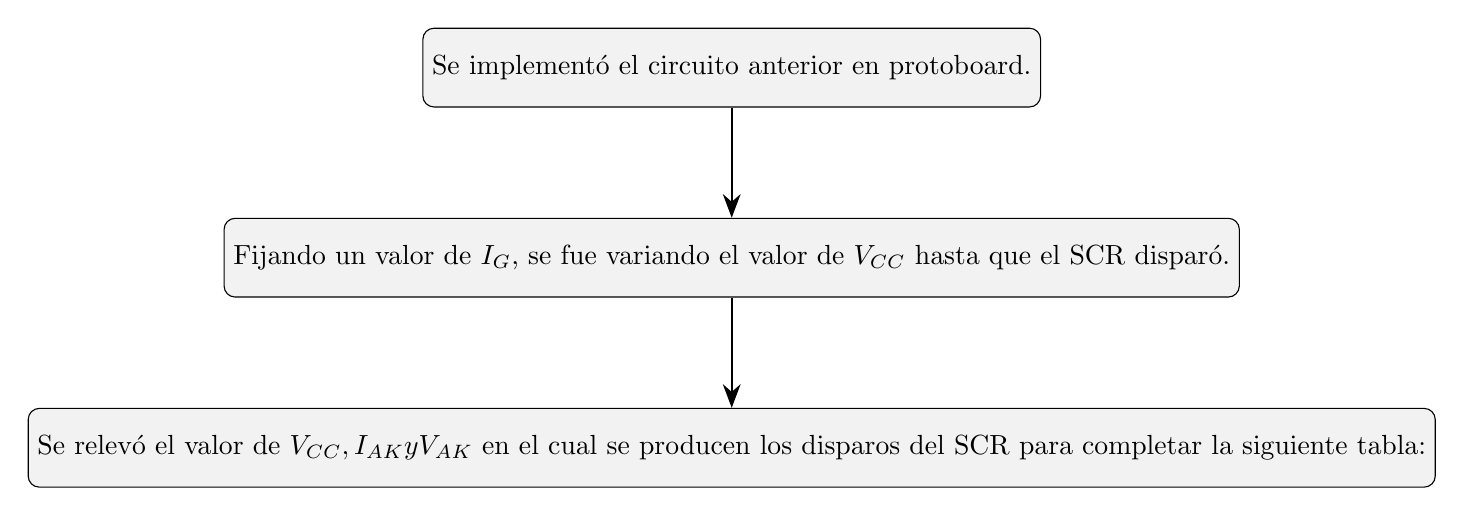
\begin{tikzpicture}[node distance=1.4cm]

\node (2) [block] {Se implementó el circuito anterior en protoboard.};
\node (3) [block, below=of 2] {Fijando un valor de $I_G$, se fue variando el valor de $V_{CC}$ hasta que el SCR disparó.};
\node (4) [block, below=of 3] {Se relevó el valor de $V_{CC}, I_{AK} \text{ y } V_{AK}$ en el cual se producen los disparos del SCR para completar la siguiente tabla:};

\foreach \i [evaluate=\i as \j using int(\i+1)] in {2,...,3}
    \draw [arrow] (\i) -- (\j);

\end{tikzpicture}\end{center}

\begin{center}
\begin{tabular}{|
>{\columncolor[HTML]{ECF4FF}}c |c|c|c|}
\hline
\cellcolor[HTML]{FFFFC7}\textbf{$I_G$ $[\mu A]$} & \cellcolor[HTML]{FFFFC7}\textbf{$V_{CC}$ $[V]$} & \cellcolor[HTML]{FFFFC7}\textbf{$I_{AK}$ $[mA]$} & \cellcolor[HTML]{FFFFC7}\textbf{$V_{AK}$ $[V]$} \\ \hline
\textbf{10}                                      &                                                 &                                                  &                                                 \\
\textbf{20}                                      &                                                 &                                                  &                                                 \\
\textbf{30}                                      &                                                 &                                                  &                                                 \\
\textbf{40}                                      &                                                 &                                                  &                                                 \\
\textbf{50}                                      &                                                 &                                                  &                                                 \\ \hline
\end{tabular}
\end{center}


\begin{center}\begin{tikzpicture}[node distance=1.4cm]

    \node (2) [block] {Fijando el valor de $I_G$, se fue variando el valor de $V_{CC}$ para relevar $I_{AK}$ y $V_{AK}$ para cada caso.};

\foreach \i [evaluate=\i as \j using int(\i+1)] in {2,...,2}
    \draw [arrow] (\i) -- (\j);

\end{tikzpicture}\end{center}
\begin{center}
\begin{tabular}{cccccccccc}
\hline
\rowcolor[HTML]{FFFFC7} 
\multicolumn{2}{|c|}{\cellcolor[HTML]{FFFFC7}$I_G = 1,47 mA$}                                                              & \multicolumn{2}{c|}{\cellcolor[HTML]{FFFFC7}$I_G = 1,59 mA$}                                                              & \multicolumn{2}{c|}{\cellcolor[HTML]{FFFFC7}$I_G = 1,74mA$}                                                               & \multicolumn{2}{c|}{\cellcolor[HTML]{FFFFC7}$I_G = 1,91 mA$}                                                              & \multicolumn{2}{c|}{\cellcolor[HTML]{FFFFC7}$I_G = 2,12 mA$}                                                              \\ \hline
\rowcolor[HTML]{FFCE93} 
\multicolumn{1}{|c|}{\cellcolor[HTML]{FFCE93}$V_{AK}$ $[V]$} & \multicolumn{1}{c|}{\cellcolor[HTML]{DAE8FC}$I_{AK}$ $[A]$} & \multicolumn{1}{c|}{\cellcolor[HTML]{FFCE93}$V_{AK}$ $[V]$} & \multicolumn{1}{c|}{\cellcolor[HTML]{DAE8FC}$I_{AK}$ $[A]$} & \multicolumn{1}{c|}{\cellcolor[HTML]{FFCE93}$V_{AK}$ $[V]$} & \multicolumn{1}{c|}{\cellcolor[HTML]{DAE8FC}$I_{AK}$ $[A]$} & \multicolumn{1}{c|}{\cellcolor[HTML]{FFCE93}$V_{AK}$ $[V]$} & \multicolumn{1}{c|}{\cellcolor[HTML]{DAE8FC}$I_{AK}$ $[A]$} & \multicolumn{1}{c|}{\cellcolor[HTML]{FFCE93}$V_{AK}$ $[V]$} & \multicolumn{1}{c|}{\cellcolor[HTML]{DAE8FC}$I_{AK}$ $[A]$} \\ \hline
\multicolumn{1}{|c|}{0}                                      & \multicolumn{1}{c|}{0}                                      & \multicolumn{1}{c|}{0}                                      & \multicolumn{1}{c|}{0}                                      & \multicolumn{1}{c|}{0}                                      & \multicolumn{1}{c|}{0}                                      & \multicolumn{1}{c|}{0}                                      & \multicolumn{1}{c|}{0}                                      & \multicolumn{1}{c|}{0}                                      & \multicolumn{1}{c|}{0}                                      \\
\multicolumn{1}{|c|}{0,3}                                    & \multicolumn{1}{c|}{190n}                                   & \multicolumn{1}{c|}{0,3}                                    & \multicolumn{1}{c|}{190n}                                   & \multicolumn{1}{c|}{0,3}                                    & \multicolumn{1}{c|}{190n}                                   & \multicolumn{1}{c|}{0,3}                                    & \multicolumn{1}{c|}{186n}                                   & \multicolumn{1}{c|}{0,3}                                    & \multicolumn{1}{c|}{186n}                                   \\
\multicolumn{1}{|c|}{0,6}                                    & \multicolumn{1}{c|}{380n}                                   & \multicolumn{1}{c|}{0,6}                                    & \multicolumn{1}{c|}{371n}                                   & \multicolumn{1}{c|}{0,6}                                    & \multicolumn{1}{c|}{371n}                                   & \multicolumn{1}{c|}{0,6}                                    & \multicolumn{1}{c|}{373n}                                   & \multicolumn{1}{c|}{0,6}                                    & \multicolumn{1}{c|}{373n}                                   \\
\multicolumn{1}{|c|}{0,9}                                    & \multicolumn{1}{c|}{2,80m}                                  & \multicolumn{1}{c|}{0,9}                                    & \multicolumn{1}{c|}{2,11m}                                  & \multicolumn{1}{c|}{0,9}                                    & \multicolumn{1}{c|}{2,1164m}                                & \multicolumn{1}{c|}{0,9}                                    & \multicolumn{1}{c|}{2,5361m}                                & \multicolumn{1}{c|}{0,9}                                    & \multicolumn{1}{c|}{2,8102m}                                \\
\multicolumn{1}{|c|}{1,2}                                    & \multicolumn{1}{c|}{2,8345m}                                & \multicolumn{1}{c|}{1,2}                                    & \multicolumn{1}{c|}{2,1288m}                                & \multicolumn{1}{c|}{1,2}                                    & \multicolumn{1}{c|}{2,1288m}                                & \multicolumn{1}{c|}{1,2}                                    & \multicolumn{1}{c|}{2,5524m}                                & \multicolumn{1}{c|}{1,2}                                    & \multicolumn{1}{c|}{2,8345m}                                \\
\multicolumn{1}{|c|}{1,5}                                    & \multicolumn{1}{c|}{2,8347m}                                & \multicolumn{1}{c|}{1,5}                                    & \multicolumn{1}{c|}{2,1290m}                                & \multicolumn{1}{c|}{1,5}                                    & \multicolumn{1}{c|}{2,1290m}                                & \multicolumn{1}{c|}{1,5}                                    & \multicolumn{1}{c|}{2,5526m}                                & \multicolumn{1}{c|}{1,5}                                    & \multicolumn{1}{c|}{2,8347m}                                \\
\multicolumn{1}{|c|}{1,8}                                    & \multicolumn{1}{c|}{2,8348m}                                & \multicolumn{1}{c|}{1,8}                                    & \multicolumn{1}{c|}{2,1292m}                                & \multicolumn{1}{c|}{1,8}                                    & \multicolumn{1}{c|}{2,1292m}                                & \multicolumn{1}{c|}{1,8}                                    & \multicolumn{1}{c|}{2,5528m}                                & \multicolumn{1}{c|}{1,8}                                    & \multicolumn{1}{c|}{2,8349m}                                \\ \hline
\multicolumn{1}{l}{}                                         & \multicolumn{1}{l}{}                                        & \multicolumn{1}{l}{}                                        & \multicolumn{1}{l}{}                                        & \multicolumn{1}{l}{}                                        & \multicolumn{1}{l}{}                                        & \multicolumn{1}{l}{}                                        & \multicolumn{1}{l}{}                                        & \multicolumn{1}{l}{}                                        & \multicolumn{1}{l}{}                                        \\
\multicolumn{1}{l}{}                                         & \multicolumn{1}{l}{}                                        & \multicolumn{1}{l}{}                                        & \multicolumn{1}{l}{}                                        & \multicolumn{1}{l}{}                                        & \multicolumn{1}{l}{}                                        & \multicolumn{1}{l}{}                                        & \multicolumn{1}{l}{}                                        & \multicolumn{1}{l}{}                                        & \multicolumn{1}{l}{}                                        \\
\multicolumn{1}{l}{}                                         & \multicolumn{1}{l}{}                                        & \multicolumn{1}{l}{}                                        & \multicolumn{1}{l}{}                                        & \multicolumn{1}{l}{}                                        & \multicolumn{1}{l}{}                                        & \multicolumn{1}{l}{}                                        & \multicolumn{1}{l}{}                                        & \multicolumn{1}{l}{}                                        & \multicolumn{1}{l}{}                                       
\end{tabular}

% \begin{tabular}{|cc|cc|cc|cc|cc|}
% \hline
% \rowcolor[HTML]{FFFFC7} 
% \multicolumn{2}{|c|}{\cellcolor[HTML]{FFFFC7}$I_G = 50\mu A$}                                             & \multicolumn{2}{c|}{\cellcolor[HTML]{FFFFC7}$I_G = 40\mu A$}                                             & \multicolumn{2}{c|}{\cellcolor[HTML]{FFFFC7}$I_G = 30\mu A$}                                             & \multicolumn{2}{c|}{\cellcolor[HTML]{FFFFC7}$I_G = 20\mu A$}                                             & \multicolumn{2}{c|}{\cellcolor[HTML]{FFFFC7}$I_G = 10\mu A$}                                             \\ \hline
% \rowcolor[HTML]{FFCE93} 
% \multicolumn{1}{|c|}{\cellcolor[HTML]{FFCE93}$V_{AK}$ $[V]$} & \cellcolor[HTML]{DAE8FC}$I_{AK}$ $[\mu A]$ & \multicolumn{1}{c|}{\cellcolor[HTML]{FFCE93}$V_{AK}$ $[V]$} & \cellcolor[HTML]{DAE8FC}$I_{AK}$ $[\mu A]$ & \multicolumn{1}{c|}{\cellcolor[HTML]{FFCE93}$V_{AK}$ $[V]$} & \cellcolor[HTML]{DAE8FC}$I_{AK}$ $[\mu A]$ & \multicolumn{1}{c|}{\cellcolor[HTML]{FFCE93}$V_{AK}$ $[V]$} & \cellcolor[HTML]{DAE8FC}$I_{AK}$ $[\mu A]$ & \multicolumn{1}{c|}{\cellcolor[HTML]{FFCE93}$V_{AK}$ $[V]$} & \cellcolor[HTML]{DAE8FC}$I_{AK}$ $[\mu A]$ \\ \hline
% \multicolumn{1}{|c|}{0}                                      &                                            & \multicolumn{1}{c|}{}                                       &                                            & \multicolumn{1}{c|}{}                                       &                                            & \multicolumn{1}{c|}{}                                       &                                            & \multicolumn{1}{c|}{}                                       &                                            \\
% \multicolumn{1}{|c|}{1}                                      &                                            & \multicolumn{1}{c|}{}                                       &                                            & \multicolumn{1}{c|}{}                                       &                                            & \multicolumn{1}{c|}{}                                       &                                            & \multicolumn{1}{c|}{}                                       &                                            \\
% \multicolumn{1}{|c|}{2}                                      &                                            & \multicolumn{1}{c|}{}                                       &                                            & \multicolumn{1}{c|}{}                                       &                                            & \multicolumn{1}{c|}{}                                       &                                            & \multicolumn{1}{c|}{}                                       &                                            \\
% \multicolumn{1}{|c|}{3}                                      &                                            & \multicolumn{1}{c|}{}                                       &                                            & \multicolumn{1}{c|}{}                                       &                                            & \multicolumn{1}{c|}{}                                       &                                            & \multicolumn{1}{c|}{}                                       &                                            \\
% \multicolumn{1}{|c|}{4}                                      &                                            & \multicolumn{1}{c|}{}                                       &                                            & \multicolumn{1}{c|}{}                                       &                                            & \multicolumn{1}{c|}{}                                       &                                            & \multicolumn{1}{c|}{}                                       &                                            \\
% \multicolumn{1}{|c|}{5}                                      &                                            & \multicolumn{1}{c|}{}                                       &                                            & \multicolumn{1}{c|}{}                                       &                                            & \multicolumn{1}{c|}{}                                       &                                            & \multicolumn{1}{c|}{}                                       &                                            \\
% \multicolumn{1}{|c|}{...}                                    &                                            & \multicolumn{1}{c|}{}                                       &                                            & \multicolumn{1}{c|}{}                                       &                                            & \multicolumn{1}{c|}{}                                       &                                            & \multicolumn{1}{c|}{}                                       &                                            \\
% \multicolumn{1}{|c|}{15}                                     &                                            & \multicolumn{1}{c|}{}                                       &                                            & \multicolumn{1}{c|}{}                                       &                                            & \multicolumn{1}{c|}{}                                       &                                            & \multicolumn{1}{c|}{}                                       &                                            \\ \hline
% \end{tabular}
\end{center}
\midTitle{blue}{Preguntas}{}

\begin{itemize}[nosep]

    \item\textbf{Conclusiones de los valores obtenidos en la primera tabla observando cómo varía el valor de $V_{CC}$ al cual se produce el disparo del SCR con cada nuevo valor de $I_G$ que se ensaya}
    \item\textbf{Graficar en el mismo par de ejes cartesianos los datos relevados en la última tabla que corresponden a la familia de curvas $I_{AK} = f(V_{AK})$ para cada diferente valor de $I_G$. Si es necesario, retome el circuito y revele a su necesidad valores intermedios que le permitan realizar una mejor curva.}

        \imagen[$I_{AK} = f(V_{AK})$ para cada $I_G$]{15cm}{./imagenes/actividadSCR/Figure_1.png}
    \item\textbf{Elavorar conclusiones del gráfico realizado.}

\end{itemize}

\subsection{Funcionamiento del SCR con corrientes alternas}
\sangria{} El objetivo de esta actividad es determinar el funcionamiento del SCR en corriente alterna y el proceso de apagado del mismo.
\subsubsection{Actividad de simulación}
\midTitle{teal}{Circuito para la simulación}{}
\begin{center}
\begin{tikzpicture}
	% Paths, nodes and wires:
	\node[oscillator](N1) at (0.73, 7.5){};
	\draw (2, 10.5) to[american resistor, l={$R_1$}] (2, 7.5);
	\draw (2, 7.5) to[american resistor, l={$R_2$}] (2, 4.5);
	\node[ground] at (2, 3.5){};
	\draw (0.25, 6) -| (0.25, 3.5) -- (2, 3.5);
	\draw (0.25, 8) -| (0.25, 10.5);
	\draw (0.25, 11.25) -- (2, 11.25);
	\draw (2, 7.5) to[american resistor, l={$R_4 [1k\Omega]$}] (4.5, 7.5);
	\draw (4.5, 7.5) to[empty diode] (6.25, 7.5);
	\draw (7.003, 9.17) to[empty thyristor, mirror] (7.023, 7.245);
	\draw (7.003, 9.17) to[american resistor, l={$R_3 [1k\Omega]$}] (7, 10.5);
	\draw (0.25, 10.5) -| (0.25, 11.25);
	\draw (2, 10.5) -| (2, 11.25);
	\draw (7, 10.5) |- (2, 11.25);
	\draw (2, 3.5) to[capacitor, l={$C 4.7\mu$}] (2, 4.75);
	\draw (0.25, 6) -| (0.25, 7);
	\draw (2, 3.5) -| (7.023, 7.245);
\end{tikzpicture}\end{center}

\midTitle{red}{Flujo de trabajo}{}
{ 
\tikzstyle{block} = [rectangle, rounded corners,
                     draw=black, fill=gray!10,
                     text width=8cm, minimum height=1cm,
                     align=center, font=\small]

\tikzstyle{arrow} = [thick, -{Latex[length=3mm,width=2mm]}]
\begin{center}
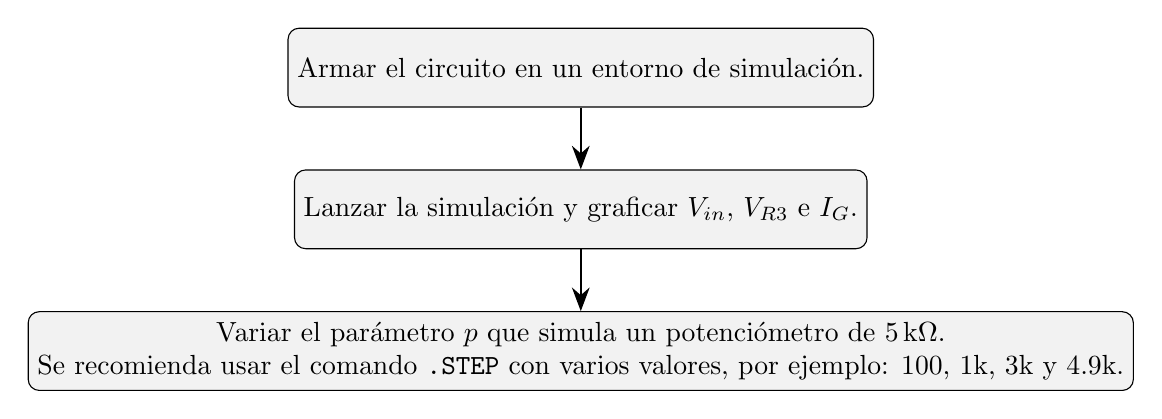
\begin{tikzpicture}[node distance=1.8cm]

\node[block] (a) {Armar el circuito en un entorno de simulación.};
\node[block, below of=a] (b) {Lanzar la simulación y graficar $V_{in}$, $V_{R3}$ e $I_G$.};
\node[block, below of=b] (c) {Variar el parámetro $p$ que simula un potenciómetro de 5\,k$\Omega$.\\
Se recomienda usar el comando \texttt{.STEP} con varios valores, por ejemplo: 100, 1k, 3k y 4.9k.};

\draw[arrow] (a) -- (b);
\draw[arrow] (b) -- (c);

\end{tikzpicture}
\end{center}

}

\midTitle{blue}{Preguntas}{}
\begin{itemize}[nosep]
    \item \textbf{Debe explicar brevemente el funcionamiento del circuito. Principalmente justificar el uso del capacitor en el circuito de la compuerta.}
\end{itemize}

\sangria{} El circuito es de un disparo de SCR con control de fase, permite regular la potencia entregada a una carga resistiva. El tiristor conduce solo durante parte del semiciclo de la señal senoidal $V_1$, al variar la fase de disparo se controla cuánta parte de la onda llega a la carga (potencia promedio se entrega). \\ \sangria{} El capacitor en la compuerta junto al divisor $R_1$ y $R_2$, con el diodo, permite retrasar el momento en el que el SCR recibe el pulso de disparo en cada semiciclo:
\begin{enumerate}[nosep]
    \item Al comienzo del semiciclo, el capacitor se carga por medio de $R_1, R_2 \text{ y } D_1$.
    \item Cuando la tensión en el capacitor alcanza la tensión de disparo del diodo y del gate del SCR, el capacitor descarga a tirra. El $Gate$ del SCR ''vió'' un pulso, por lo que se enciende.
    \item La carga queda conectada al suministro hasta que la corriente de línea cae a cero (sería el fin del semiciclo).\\
\end{enumerate}
\sangria{} El potenciometro modifica la constante de tiempo $\tau = R_{eq} \cdot C_1$. Así controla cuánto tarda el capacitor en cargarse y por lo tanto, en qué punto del semiciclo dispara el SCR:

\begin{itemize}[nosep]
    \item Menor resistencia $\rightarrow$ el capacitor carga más rápido $\rightarrow$ El SCR se dispara antes y hay más potencia en la carga.
    \item Mayor resistencia $\rightarrow$ el capacitor se carga más lento $\rightarrow$ El SCR dispara más tarde y hay menos potencia en la carga.\\[5pt]
\end{itemize}



\begin{itemize}[nosep]
    \item \textbf{Tome una de las simulaciones y analice las corrientes $I_G$ en el momento de disparo y la corriente $I_{AK}$ en el momento de apagado ¿Coincide con el valor esperado?}
\end{itemize}

\imagen[Corriente en el $Gate$ del SCR]{15cm}{./imagenes/actividadSCR/I_G_disparo_scr.png}
\sangria{} Nótese cómo en milisegundos, la corriente en el $Gate$ sube hasta cierto valor hasta que el capacitor termina de cargarse y se descarga a tierra. Por lo que el $Gate$ ve un pulso de corriente lo suficiente para activdar el SCR.

\imagen[Sinuidal de la fuente]{15cm}{./imagenes/actividadSCR/formaSinuidalUltimoSCR.png}

\imagen[Corriente ánodo cátodo para distintos valores de $R_2$]{15cm}{./imagenes/actividadSCR/corrienteIAKUltimoSCR.png}

\sangria{} Nótese que, para $R_2 = 0$, la onda sinuidal de la fuente entra casi completa a la carga y a medida que aumenta, entran solo ciertos semiciclos de la fuente (porque el capacitor se carga instantáneamente).

\begin{itemize}[nosep]
    \item \textbf{Identificar el ángulo mínimo y máximo que puede controlar. Exprese en grados ($\text{}^o$)}
\end{itemize}


